\documentclass[14pt,russian,utf8]{extarticle}
\usepackage{repstyle}
\begin{document}


\section {Реализованные алгоритмы}
\subsection{Алгоритм нахождения мел-частотных кепстральных коэффициентов}


Запишем исходный речевой сигнал как  
\[
	x_{n}, \; \; 0 \leq n < N 
	\eqno{(1)}
\]

Получим спектр сигнала, используя ДПФ
\[
	X_{k}=\sum_{n=0}^{N-1}{x_{n}e^{\frac{-2\pi i}{N}kn}}, \; \;  0 \leq k < N
	\eqno{(2)}
\]

Определим оконные функции. В данном случае использованы M треугольных окон, равномерно расположенные относительно мел-шкалы
\[
	H_{m}=
	\begin{cases}
		0,&k<f_{m-1}\\ 
		\frac{(k-f_{m-1})}{(f_{m}-f_{m-1})},&f_{m-1} \leq k < f_{m}\\ 
		\frac{(f_{m+1}-k)}{(f_{m+1}-f[m])},&f_{m} \leq k \leq f_{m+1}\\ 
		0,&k > f_{m+1}
\end{cases}
\eqno{(3)}
\]

Граничные частоты $f_{m}$ получены из равенства
\[
	f_{m}=(\frac{N}{F_{s}})\cdot B^{-1}(B(f_{1})+m\frac{B(f_{в})-B(f_{1})}{M+1}), \; \; 0 \leq m < M
	\eqno{(4)}
\]

где $B(f)$ --- операция перевода значений частоты в мел-шкалу
\[
	B(f)=1125\ln(1+f/700)
	\eqno{(5)}
\]

Соответственно, обратная операция
\[
	B^{-1}(b)=700(exp(b/1125)-1)
	\eqno{(6)}
\]

\begin{figure}[H]
	\begin{multicols}{2}
		\hfill
		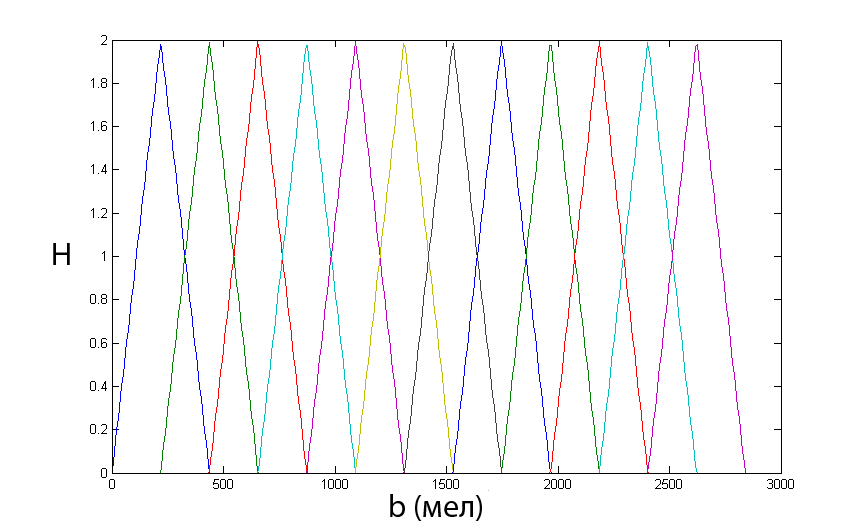
\includegraphics[width=85mm]{graph-3.png}
			%\hfill
			\caption{Окна (мел-шкала)}
			\label{wind-mel}
			%\hfill
		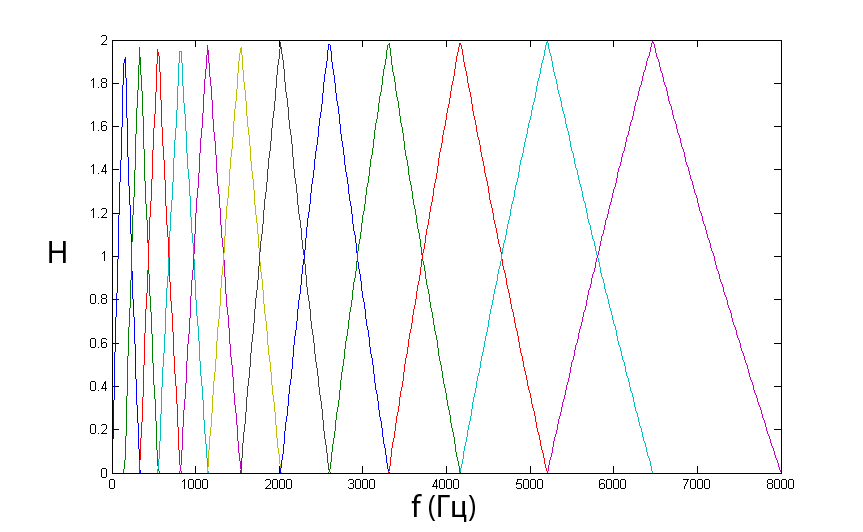
\includegraphics[width=85mm]{graph-4.png}
			%\hfill
			\caption{Окна (частотная шкала)}
			\label{wind-hz}
	\end{multicols}
\end{figure}

Вычислим логарифм значения энергии сигнала для каждого окна анализа
\[
	S_{m}=ln(\sum_{k=0}^{N-1}{|X_{k}|^{2}H_{m,k})}, \; \; 0\leq m<M
	\eqno{(7)}
\]

Чтобы получить набор мел-частотных кепстральных коэффициентов, к полученным значениям применим ДКП
\[
	c_{n}=\sum_{m=0}^{M-1}{S_{m}cos(\pi n(m+1/2)/M)}, \; \; 0\leq n < M
	\eqno{(8)}
\]

Полученные в результате значения, а также их изменения во времени, используются в дальнейшем как описание речевого сигнала.
\pagebreak

\subsection{Алгоритм сравнения речевых сигналов с применением динамического программирования (DTW)}

Алгоритм динамического трансформирования времени (DTW) вычисляет оптимальную последовательность трансформации (деформации) времени между двумя временными рядами. Алгоритм вычисляет оба значения деформации между двумя рядами и расстоянием между ними. 


Предположим, что есть две числовые последовательности $A= a_{1}, a_{2}, \dots, a_{I}$ и $B=b_{1}, b_{2}, \dots, b_{J}$. Длина двух последовательностей может быть различной.

Временные различия между A и B могут быть описаны с помощью некоторой последовательности $c=(i,j)$:
\[
	F=c(1),c(2)\dots,c(k),\dots,c(K)
	\eqno{(9)}
\]
где $c(k)=(i(k),j(k))$.
Данная последовательность представляет собой функцию, которая позволяет отобразить временную ось A на временной оси B. Назовем ее функцией деформации. \cite{sakoechiba}

\begin{figure}[H]	
	\centering
	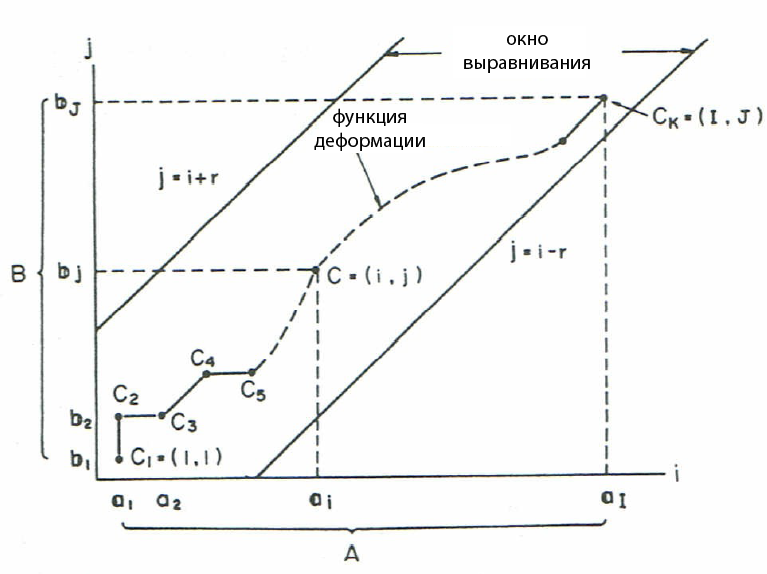
\includegraphics[width=120mm]{sakoe1.png}			
	\caption{Функция деформации и окно выравнивания}
	\label{sakoe1}
\end{figure}

Алгоритм начинается с расчета локальных расстояний между элементами двух последовательностей. Самый распространенный способ для вычисления расстояний является метод, рассчитывающий модуль разности между значениями двух элементов (Евклидова метрика). В результате получаем матрицу расстояний, имеющую I строк и J столбцов общих членов:
\[
d(c)=d(i,j)=|a_{i}-b_{j}|, i=1..I, j=1..J
\eqno{(10)}
\]

Взвешенная сумма значений метрик в точках, принадлежащих функции деформации F
\[
E(F)=\sum_{k=1}^{K}{d(c(k))\cdot w(k)}
\eqno{(11)}
\]
(где $w(k)$ - неотрицательный весовой коэффициент) является мерой доброкачественности функции F. Она принимает минимальное значение, когда функция F оптимально выравнивает временные различия между A и B. Минимальное остаточное расстояние между A и B, которое остается после устранения временных различий, может служить мерой различия речевых последовательностей A и B
\[
D(A,B)=min_F\left[\frac{\sum_{k=1}^{K}{d(c(k))\cdot w(k)}}{\sum_{k=1}^{K}{w(k)}}\right]
\eqno{(12)}
\]


Существует три условия, налагаемых на DTW алгоритм для обеспечения быстрой конвергенции:

\begin{enumerate}
 \item Монотонность – путь никогда не возвращается, то есть: оба индекса, i и j, которые используются в последовательности, никогда не уменьшаются. 

 \item Непрерывность – последовательность продвигается постепенно: за один шаг индексы i и j, увеличиваются не более чем на 1.

 \item Предельность – последовательность начинается в (1,1) и заканчивается в (I,J).
 \end{enumerate}

Практическая реализация данного алгоритма представляет собой нахождение значения нормированного расстояния
\[
D(A,B)=\frac{1}{N}g_{K}(c(K))
\eqno{(13)}
\]
где $g_{k}(c(k))$ можно найти из уравнения:
\[
g_{k}(c(k))=\min_{c(k-1)}[g_{k-1}(c(k-1))+d(c(k))\cdot w(k)]
\eqno{(14)}
\]

Начальное условие:
\[
g_{1}(c(1))=d(c(1))\cdot w(1)
\eqno{(15)}
\]

Из ограничений следует, что $c(1)=(1,1)$,
\[
g(i,j)=\min \left[ \begin{matrix} g(i,j-1)+d(i,j) & \\ g(i-1,j-1)+2d(i,j) &\\ g(i-1,j)+d(i,j) &\end{matrix} \right].
\eqno{(16)}
\]

В данном случае нормированное расстояние можно записать как
\[
D(A,B)=\frac{1}{K}g(I,J), \text{где K - размерность вектора $c$.}
\eqno{(17)}
\]
\begin{figure}[H]	
	\centering
	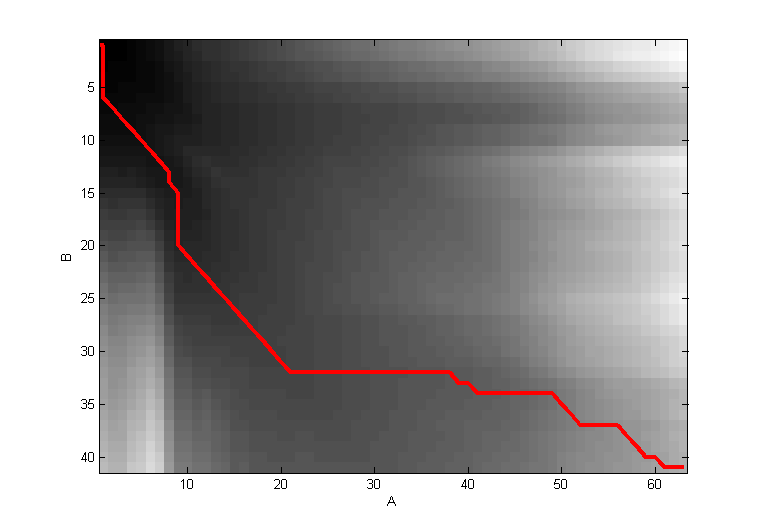
\includegraphics[width=120mm]{d_matrix.png}			
	\caption{Пример нахождения функции деформации}
	\label{d_matrix1}
\end{figure}

Эксперименты проводились для словаря из 10 слов (цифры от 0 до 9). Одним диктором было записано 100 повторений для сравнения (по 10 для каждого в словаре).


С помощью данного алгоритма производится сравнение анализируемого сигнала с сохраненными в памяти компьютера эталонами. В результате выбирается пара с минимальной дистанцией и делается вывод о соответствии сигнала слову из словаря. Результат сравнения слова <<четыре>> со словарем можно видеть на рис. \ref{distances_4} (Меньшее значение дистанции означает большее сходство).

\begin{figure}[H]	
	\centering
	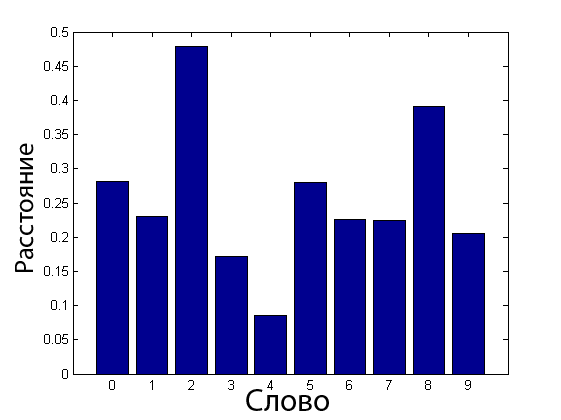
\includegraphics[width=120mm]{distances_4.png}			
	\caption{Диаграмма расстояний для слова <<четыре>>}
	\label{distances_4}
\end{figure}

В результате, на 100 повторений было обнаружено 2 ошибки распознавания, что позволяет говорить о достаточной точности выбранного алгоритма. На рис. \ref{dist_err_8} показана диаграмма расстояний для ошибочно распознанного слова <<восемь>>

\begin{figure}[H]	
	\centering
	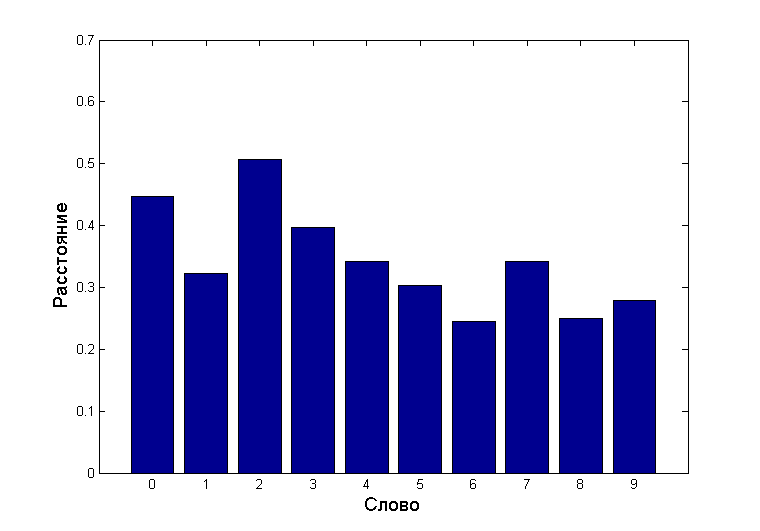
\includegraphics[width=120mm]{err_8.png}			
	\caption{Диаграмма расстояний для ошибочно распознанного слова <<восемь>>}
	\label{dist_err_8}
\end{figure}

\pagebreak
\begin{thebibliography}{9}
	\bibitem{vincuk}
	Винцюк Т.К. Анализ, распространение и интерпретация речевых сигналов. Киев: Наукова думка, 1987.
	\bibitem{spokenlangproc}
	Xuedong Huang, Alex Acero, Hsiao-Wuen Hon, Spoken Language Processing: A Guide to Theory, Algorithm, and System Development, Prentice Hall, 2001, ISBN:0130226165
	\bibitem{sakoechiba}
	H. Sakoe and S. Chiba, <<Dynamic programming optimization for spoken word recognition>>, IEEE   Trans.  Acoust. Speech  Signal  Process.,  Vol. ASSP-26, No. 1, Feb. 1978
	\bibitem{mazurenko}
	 Мазуренко И.Л. Компьютерные системы распознавания речи. Интеллектуальные системы, Москва, 1998 г.
	\bibitem{lindsay}
	 П. Линдсей, Д. Норман Переработка информации у человека — М: Мир, 1974
\end{thebibliography}

\end{document}